\documentclass[14pt, a4paper, titlepage]{extarticle}
\usepackage{style}
\usepackage{lipsum}

\title{Лабораторные работы по компьютерной графике}
\author{Максимов П.А.}

\begin{document}

	\maketitle

	\tableofcontents

	\pagebreak

	Данный документ включает в себя информацию по лабораторным работам по компьютерной графике. Суть лабораторных работ заключается в поэтапном написании графического движка, основанного на технологии \textit{Raycast}. 

	\section{Лабораторная работа №1: Базовая алгебра и геометрия проекта}
	Первая лабораторная работа заключается в реализации базовых классов линейной алгебры и аналитической геометрии.

\subsection{Определения}

	Определим понятие линейного (векторного) пространства и базиса. 

	\textit{Линейное (векторное) пространство} -- множество векторов, в котором определены операции сложения и умножения на число.

	\textit{Базис} -- полная система линейно независимых векторов линейного пространства. В ней ни один из векторов нельзя выразить линейно через другие, и через них можно описать любой вектор линейного пространства.
	
	\textit{Система координат} -- система, состоящая из произвольной начальной точки и базиса. 

	В линейном пространстве задается скалярное произведение. Свойства скалярного произведения:
	\begin{enumerate}
		\item \( \pares{\ua, \ub} = \pares{\ub, \ua} \) -- симметричность;
		\item \( \pares{k \ua, \ub} = k\pares{\ua, \ub}, ~ k - \mathrm{const} \) -- линейность;
		\item \( \pares{\ua + \ub, \uc} = \pares{\ua, \ub} + \pares{\ub, \uc} \) -- дистрибутивность.
	\end{enumerate} 

	Выразим скалярное произведение через координаты перемножаемых векторов. Пусть \( \uf_1, \uf_2, \dots \uf_n \) -- базис пространства векторов, и \( \ua = \alpha_1 \uf_1 + \alpha_2 \uf_2 + \dots + \alpha_n \uf_n \), \( \ub = \beta_1 \uf_1 + \beta_2 \uf_2 + \dots + \beta_n \uf_n \) -- разложение векторов $\ua, \ub$ по этому базису. Тогда по свойствам скалярного произведения получаем:
	\[ \pares{\ua, \ub} = \sum_{i, j = 1}^{n} \alpha_i \beta_j \pares{\uf_i, \uf_j} \]
	Обозначим матрицу Грама
	\[ 
		\Gamma \pares{\uf_1, \uf_2, \dots, \uf_n} = 
		\begin{pmatrix} 
			\pares{\uf_1, \uf_1}_*, & \cdots & \pares{\uf_1, \uf_n}_* \\ 
			\vdots & \ddots & \vdots \\ 
			\pares{\uf_n, \uf_1}_* & \cdots & \pares{\uf_n, \uf_n}_*
		\end{pmatrix}
	\]
	и координаты вектора $\uv$ в базисе $f$:
	\( \bracks{\uv}_f = \begin{pmatrix} v_1 \\ \vdots \\ v_n \end{pmatrix}. \)
	
	Здесь \( \pares{\ua, \ub}_* = \sum\limits_{k=1}^n a_k b_k \) -- диагональная билинейная форма скалярного произведения (в ортонормированном базисе).

	Тогда скалярное произведение в неортонормированном базисе $f$ можно представить с помощью матричного умножения:
	\[ \pares{\ua, \ub}_{f} = \bracks{\ua}^{T} \cdot \Gamma\pares{\uf_1, \dots, \uf_n} \cdot \bracks{\ub}_f. \]

	Билинейной формой будем называть такую функцию двух аргументов, которая будет линейной относительно них, и удовлетворяет следующим свойствам:
	\begin{enumerate}
		\item \( F(x + z, y) = F(x, y) + F(z, y) \);
		\item \( F(x, y + z) = F(x, y) + F(x, z) \);
		\item \( F(kx, y) = F(x, ky) = k F(x, y), ~ k - \mathrm{const} \).
	\end{enumerate}

	Классическим случаем билинейной формы считаются функции двух $n$-мерных векторов линейного пространства следующего вида:
	\[ F(\ux, \uy) = \sum_{i, j=1}^{n} a_{ij} x_i y_j.  \]

	Ортонормированным векторным произведением будем называть следующую конструкцию:
	\[ 
		\bracks{\underline{u}, \underline{v}} = \det\begin{vmatrix} \underline{i} & \underline{j} & \underline{k} \\ u_x & u_y & u_z \\ v_x & v_y & v_z \end{vmatrix}; 
		\quad \underline{i} = \begin{pmatrix} 1 \\ 0 \\ 0 \end{pmatrix}, 
		~ \underline{j} = \begin{pmatrix} 0 \\ 1 \\ 0 \end{pmatrix}, 
		~ \underline{k} = \begin{pmatrix} 0 \\ 0 \\ 1 \end{pmatrix}. 
	\]

	Векторным произведением в трехмерном пространстве с косоугольным базисом \( \bracs{\underline{b}_1, \underline{b}_2, \underline{b}_3} \) будем называть следующее выражение:
	\[ 
		\bracks{\underline{u}, \underline{v}}_{*} = \det\begin{vmatrix} \bracks{\underline{b}_2, \underline{b}_3} & \bracks{\underline{b}_3, \underline{b}_1} & \bracks{\underline{b}_1, \underline{b}_2} \\ u_x & u_y & u_z \\ v_x & v_y & v_z \end{vmatrix}.
	\]

\subsection{Этапы реализации}

	Зафиксируем представленную алгебру и геометрию в поэтапной реализации движка:
	\begin{enumerate}
		\item Реализация класса матрицы и функции билинейной формы. Их будем считать самыми первостепенными классами нашего движка.
		\item На основе матрицы реализуем понятие радиус-вектора. Для них реализуем скалярное и векторное (только для трехмерного случая) произведения в ортонормированном пространстве.
		\item Для класса матрицы с помощью билинейной формы реализуем матрицу Грама, принимающую на себя $n$ векторов размерности $n$.
		\item Введем понятие векторного пространства с базисом, внутри которого реализуем скалярное и векторное произведения на основе рассматриваемого базиса.
		\item Реализуем понятие точки в векторном пространстве на основе понятия вектора.
		\item На основе точек и векторного пространства реализуем систему координат.
	\end{enumerate}

\subsection{Класс Matrix}
	\noindent Класс матрицы, содержащий базовые алгебраические операции над матрицами.

	\noindent Инициализация:
	\begin{enumerate}
		\item \inlinecode{Matrix(n: int)} -- нулевая матрица заданной размерности \( n \times n \);
		\item \inlinecode{Matrix(n: int, m: int)} -- нулевая матрица заданной размерности \( n \times m \);
		\item \inlinecode{Matrix(elements: list[list[int | float]])} -- матрица с заданными элементами.
	\end{enumerate}

	\noindent Реализуемые поля:
	\begin{enumerate}
		\item \inlinecode{n(int), m(int)} -- размерность матрицы;
		\item \inlinecode{elements(list[list[matrix(float)]])} -- массив матрицы.
	\end{enumerate}

	\noindent Реализуемые методы:
	\begin{enumerate}
		\item \inlinecode{addition(m: Matrix) -> Matrix}, \inlinecode{multiplication(m: Matrix) -> Matrix}, \newline \inlinecode{multiplication(c: int | float) -> Matrix} -- базовые матричные операции;
		\item \inlinecode{get_minor(lines: list[int], rows: list[int]) -> Matrix} -- создает матрицу, основанную на текущей, из которой исключаются заданные строки и столбцы;
		\item \inlinecode{determinant() -> float} -- определитель матрицы (работает только в случае \(n \times n\));
		\item \inlinecode{inverse() -> Matrix} -- обратная матрица (работает только в случае \(n \times n\) и \( \det{A} \neq 0 \));
		\item \inlinecode{transpose() -> Matrix} -- транспонированная матрица;
		\item \inlinecode{norm() -> float} -- норма матрицы;
		\item \inlinecode{Matrix.identity(n: int) -> Matrix} -- статический метод, создающий $n$-мерную единичную матрицу;
		\item \inlinecode{Matrix.gram(v1, ..., vn : Vector) -> Matrix} -- статический метод, создающий матрицу Грама на основе заданных $n$-векторов размерности $n$.
	\end{enumerate}

	\noindent Перегружаемые операторы:
	\begin{enumerate}
		\item \inlinecode{Matrix + | - Matrix} (операции сложения и вычитания матриц);
		\item \inlinecode{Matrix * [Matrix | int | float]} (левое и правое умножение, умножение слева перегрузить на основе умножения справа);
		\item \inlinecode{Matrix / [Matrix | int | float]} (на основе метода \inlinecode{inverse});
		\item \inlinecode{\~ Matrix} (обращение матрицы через \inlinecode{inverse});
		\item \inlinecode{Matrix[i, j : int] | Matrix[i: int][j: int]} (операция обращения (и присваивания) к элементу матрицы).
	\end{enumerate}

\subsection{Функция BilinearForm(\textit{Matrix, Vector, Vector})}
	\noindent Функция принимает на себя матрицу $n \times n$, и два вектора размерности $n$. Возвращает результат рассчета билинейной формы относительно двух векторов.

\subsection{Класс Vector[\textit{Matrix}]}
	\noindent Класс вектора наследуется от класса матрицы, является частным случаем матрицы $n \times 1$.

	\noindent Инициализация:
	\begin{enumerate}
		\item \inlinecode{Vector(n: int)} -- нулевой вектор заданной размерности \( n \);
		\item \inlinecode{Vector(elements: list[list[int | float]])} -- вектор-столбец с заданными значениями;
		\item \inlinecode{Vector(elements: list[int | float])} -- вектор-строка с заданными значениями.
	\end{enumerate}

	\noindent Реализуемые методы:
	\begin{enumerate}
		\item \inlinecode{scalar_product(v1, v2 : Vector) -> float} -- ортонормированное скалярное произведение двух $n$-мерных векторов;
		\item \inlinecode{vector_product(v1, v2 : Vector) -> Vector} -- ортонормированное векторное произведение двух трехмерных векторов (через определитель матрицы);
		\item \inlinecode{length() -> float} -- длина вектора;
		\item \inlinecode{normalize() -> Vector} -- нормализация вектора;
		\item \inlinecode{dim() -> int} -- размерность вектора.
	\end{enumerate}

	\noindent Перегружаемые операторы:
	\begin{enumerate}
		\item \inlinecode{Vector \% Vector} (ортонормированное скалярное произведение);
		\item \inlinecode{Vector ^ | ** Vector} (ортонормированное векторное произведение (только для трехмерного случая));
		\item \inlinecode{Vector[i: int]} (операция обращения к элементу вектора, вне зависимости от алгебраической формы -- строка или столбец).
	\end{enumerate}

\subsection{Класс VectorSpace}
	\noindent Класс векторного пространства, содержащего набор базисных векторов.

	\noindent Инициализация:
	\begin{enumerate}
		\item \inlinecode{VectorSpace(basis: list[Vector])} -- векторное пространство с заданными базисными векторами.
	\end{enumerate}

	\noindent Реализуемые поля:
	\begin{enumerate}
		\item \inlinecode{basis(list[Vector])} -- список базисных векторов.
	\end{enumerate}

	\noindent Реализуемые методы:
	\begin{enumerate}
		\item \inlinecode{scalar_product(v1, v2 : Vector) -> float} -- скалярное произведение двух $n$-мерных векторов в базисе данного пространства;
		\item \inlinecode{vector_product(v1, v2 : Vector) -> Vector} -- векторное произведение двух 3-мерных векторов в базисе данного пространства;
		\item \inlinecode{as_vector(pt: Point) -> Vector} -- вектор, полученный разложением координат точки по базисным векторам.
	\end{enumerate}

\subsection{Класс Point[\textit{Vector}]}
	\noindent Класс точки, являющейся частным случаем вектора. 

	\noindent Инициализация:
	\begin{enumerate}
		\item \inlinecode{Point} -- наследуемая инициализация согласно инициализации вектора;
		\item \inlinecode{Point(vec: Vector)} -- точка на основе вектора.
	\end{enumerate}

	\noindent Перегружаемые операторы:
	\begin{enumerate}
		\item \inlinecode{Point + | -- Vector} (перенос точки).
	\end{enumerate}

	Наследованные операторы умножения и деления необходимо упразднить.

\subsection{Класс CoordinateSystem}
	\noindent Класс системы координат, содержащей начальную точку и базисные вектора.

	\noindent Инициализация:
	\begin{enumerate}
		\item \inlinecode{CoordinateSystem(initial: Point, basis: VectorSpace)} -- система координат с начальной точкой и базисом.
	\end{enumerate}

	\noindent Реализуемые поля:
	\begin{enumerate}
		\item \inlinecode{initial_point(Point)} -- начальная точка системы координат;
		\item \inlinecode{space(VectorSpace)} -- базисные вектора.
	\end{enumerate}
		
	\pagebreak
	\section{Лабораторная работа №2: Автоматическое тестирование и исключения}
	Вторая лабораторная работа заключается в реализации преобразований поворота на основе частного случая углов Эйлера, реализация класса исключений для движка, и написания автотестов. 

\subsection{Определения}

	Определим частный случай поворотов с помощью углов Эйлера -- углы поворота Тейта-Брайана. Для начала введем понятие матрицы поворота в двумерном пространстве.

	Матрицей поворота в двумерном пространстве называется матрица следующего вида:
	\[ R \pares{\alpha} = \begin{pmatrix} \cos{\alpha} & -\sin{\alpha} \\ \sin{\alpha} & \cos{\alpha} \end{pmatrix}. \]
	Данная матрица при применении на любой вектор в правосторонней системе координат совершает поворот представленного вектора <<против часовой стрелке>> на заданный угол $\alpha$. В трехмерном случае такую матрицу можно применить в поворотах относитель трех пар координатных осей: XY, YZ, XZ. Для каждой пары согласно четности перестановки матрицы поворота вокруг соответствующих осей будут иметь следующий вид:
	\[ 
		R_x \pares{\alpha} = 
		\begin{pmatrix} 
			1 & 0 & 0 \\ 
			0 & \cos{\alpha} & -\sin{\alpha} \\ 
			0 & \sin{\alpha} & \cos{\alpha} 
		\end{pmatrix}
	\] 
	\[
		R_y \pares{\beta} = 
		\begin{pmatrix} 
			\cos{\beta} & 0 & \sin{\beta} \\ 
			0 & 1 & 0 \\ 
			-\sin{\beta} & 0 & \cos{\beta}
		\end{pmatrix} 
	\]
	\[ 
		R_z \pares{\gamma} = 
		\begin{pmatrix} 
			\cos{\gamma} & -\sin{\gamma} & 0 \\ 
			\sin{\gamma} & \cos{\gamma} & 0 \\ 
			0 & 0 & 1
		\end{pmatrix}
	\]
	Общее преобразование поворота на углы $\alpha, \beta, \gamma$ вокруг осей $Ox, Oy, Oz$ согласно поворотам Тейта-Брайана будет принимать следующий вид:
	\[ R_{x, y, z} \pares{\alpha, \beta, \gamma} = R_x \pares{\alpha} \cdot R_y \pares{\beta} \cdot R_z \pares{\gamma}. \]

\subsection{Исключения}

	Теперь перейдем к разделу исключений. Для реализации движка желательно реализовать собственные подклассы исключений для различных разделов игрового движка. Это необходимо для более точечной классификации ошибок работы движка. В качестве рекомендации предлагается ввести общий класс исключений (например, \inlinecode{EngineException}), относительно которого создать отдельные подклассы исключений для различных случаев (например, \inlinecode{MatrixException}). Внутри каждого отдельного класса исключений можно задать распространенные тексты ошибок в виде полей или методов класса:

	\begin{figure}[H]
		\begin{lstlisting}[caption=<<Пример (Python)>>]
class EngineException(Exception):
	pass

class MatrixException(EngineException):
	MATRIX_UNKNOWN_OPERATION = "This operation isn't defined for matrix"

	@staticmethod
	def MATRIX_WRONG_SIZES(n1: int, m1: int, n2: int, m2: int) -> str:
		return f"Wrong sizes: {n1}x{m1} and {n2}x{m2}"

class VectorException(EngineException):
	VECTOR_UNKNOWN_OPERATION = "This operation isn't defined for vector"
		\end{lstlisting}
	\end{figure}

	Также возможен и другой вариант. Для каждого варианта исключения можно оформить свой класс (с сообщением, которое затем вызывать):
	\begin{figure}[H]
		\begin{lstlisting}[caption=<<Пример (Python)>>]
class EngineException(Exception):
	pass

class MatrixWrongSizeException(EngineException):
	@staticmethod
	def MESSAGE(n1: int, m1: int, n2: int, m2: int) -> str:
		return f"Wrong sizes: {n1}x{m1} and {n2}x{m2}"

class MatrixIncorrectOperationException(EngineException):
	MESSAGE = "Incorrect operation"
		\end{lstlisting}
	\end{figure}


\subsection{Модульное тестирование}

	Теперь по поводу модульного тестирования. Такое тестрование необходимо для больших проектов для проверки модулей на работоспособность при внесении в них каких-либо изменений. В нашем движке необходимо реализовать тесты на все реализуемые модули. Для упрощения написания тестов можно воспользоваться уже готовыми фреймворками, которые, к примеру, могут быть интегрированы в среду разработки.

	Рассмотрим некоторые примеры фреймворков:
	\begin{enumerate}
		\item <<C++>> -- <<GTest>>, <<Catch2>>, и др.;
		\item <<Python>> -- <<pytest>>;
		\item <<Java>> -- <<JUnit>>;
		\item <<C\#>> -- <<MS Test>>;
		\item <<Rust>> -- встроенная утилита <<cargo test>>
	\end{enumerate}

	Обсудим вопрос наименований и самой логики тестирования. Как было сказано ранее, тестирование должно проводиться для каждого модуля индивидуально, соотвественно название модуля тестирования можно писать через название с подписью <<Tests>>: \inlinecode{LowLevelClasses.Tests}. Для каждого модуля создаем классы, содержащие говорящие названия того, что тестируется, и подписью <<Tests>>: \inlinecode{MatrixOperationsTests}, \inlinecode{VectorOperationsTests}. Внутри классов задаем методы с названием, в котором отображается суть теста. Также стоит придерживаться единого метода написания тестов. Более простым и очевидным методом считается метод <<Arrange -- Act -- Assert>>, в котором код каждого теста разделяется на три основные части по следующему принципу:
	\begin{enumerate}
		\item <<Arrange>> -- Настройка тестового окружения, введение переменных, с которыми будем работать;
		\item <<Act>> -- Выполнение действия, которое необходимо протестировать с заданными переменными;
		\item <<Assert>> -- Проверка того, что выполненное действие является корректным.
	\end{enumerate} 

	\begin{figure}[H]
		\begin{lstlisting}[caption=<<Пример (Python)>>]
#File: LowLevelOperations.Tests
class MatrixOperationsTests:
	def MatrixAddition(self):
		#Arrange
		matrix1 = Matrix([[1, -1], [-1, 1]])
		matrix2 = Matrix([[0, 1], [1, 0]])
		matrix3 = Matrix([[1, 0], [0, 1]])

		#Act
		result = matrix1 + matrix2

		#Assert
		assert result == matrix3
		\end{lstlisting}
	\end{figure}

	Также к рекоммендациям можно отнести выделенное тестирование -- тестируем ровно одну операцию за один раз.

\subsection{Документация}

	Для проекта рекоммендуется ввести документацию. Она включает в себя детальное описание реализуемых модулей с примерами применения тех или иных частей проекта в реализации. В качестве примера можно привести любую документацию к языкам программирования.

	Реализация документации производится на странице Wiki пользовательского репозитория проекта на сервисах <<GitHub>> (\textit{только в публичных репозиториях}) или <<GitLab>>. Страницы распределяются по классам. Если классы содержат не так много документируемой информации, при этом являются смежными классами, то их можно объединить на одной странице. Документация предпочтительно может быть написана на английском языке, но и вариант с русским языком также возможен. В дополнение, код так же должен быть задокументирован в самом исходном коде каждого модуля. Реализация документирования внутри исходного кода является индивидуальной для каждого языка.

	Страница должна содержать следующую информацию:
	\begin{enumerate}
		\item Название класса (или обобщение названия для смежного набора классов);
		\item Краткая характеристика класса/классов -- информация о странице, о том, что описывается, и другое;
		\item Информация о том, как импортируется модуль с данными классами;
		\item Информация о классе/классах -- инициализация, список полей, список методов (в логическом порядке), список перегруженных операторов. Для каждого поля, метода и оператора прописать полагаемые типы данных на входе, и ожидаемый тип данных на выходе;
		\item Примеры использования с выводом (в виде комментария).
	\end{enumerate}

	\begin{figure}[H]
		\begin{lstlisting}[language=XML, caption=Краткий пример страницы <<Matrix>> на языке <<Markdown>>]
This page contains information about class `Matrix`. Matricies are basic algebraic objects, used in math...

#Initialization:
Possible variants for initialization:
- `Matrix(n: int, m: int)` &mdash; creates zero matrix with `n` rows and `m` columns;
- `Matrix(elements: list[list[any]])` &mdash; creates matrix with default values;
...

#Attributes:
- `n: int`, `m: int` &mdash; count of matrix rows and columns;
- `data: list[list[any]]` &mdash; matrix data;
...

#Methods:
- `set_value(i: int, j: int, value: any) -> None` &mdash; method sets value for `i` row and `j` column;
- `determinant() -> float` &mdash; method called for square matrix, which return its determinant;
- `Matrix.identity(n: int) -> Matrix` &mdash; static method which returns square identity matrix with size `n`;
...

#Overloaded:
- `Matrix + Matrix -> Matrix` &mdash; matrix addition operator;
- `Matrix * Matrix | int | float -> Matrix` &mdash; matrix multiplication operator;
...

#Examples
Example 1: Matrix initialization, multiplication and determinant usage
```Python
matrix1 = Matrix([[1, 0, 1], [0, 1, 2]])
matrix2 = Matrix([[-1, 2], [0, 1], [2, -3]])

matrix3 = matrix1*matrix2 # Matrix([[1, -1], [4, -5]])
matrix4 = matrix2*matrix3 # Matrix([[-1, 2, 3], [0, 1, 2], [2, -3, -4]])

print(matrix3.determinant(), matrix4.determinant())
# Result: -1, 0
```

Example 2: Something...
		\end{lstlisting}
	\end{figure}

	Также, документацию можно оформить отдельными файлами в заданной папке документации, описывающей индивидуально каждую страницу.


	% \textit{\lipsum[1]}

\subsection{Этапы реализации}

	Зафиксируем представленную информацию:
	\begin{enumerate}
		\item Разделим весь проект на модули. Классы, отвечающие за математическое составляющее движка необходимо вынести в отдельный файл, так же другие части движка, такие как исключения нужно вынести отдельно.
		\item В класс матриц введем операции поворота относительно осей с помощью преобразований углов Тейта-Брайана.
		\item Введем собственный класс исключений на основе базового класса, который будет содержать необходимые поля и методы для реализации выводов именованых исключений в модулях.
		\item Проведем модульное тестирование для уже готовых классов. Тестирование должно быть структурировано таким образом, чтобы оно затрагивало все созданные операции в модуле. Важно обратить внимание на наименование файлов, классов и методов в тесте.
		\item Введем документацию, содержащую информацию о классах, их полях и методах, зависимостях. В документации реализуем список изменений.

	\end{enumerate}

	В дальнейшем сдача лабораторных работ будет производиться по следующим критериям:
	\begin{enumerate}
		\item Список изменений с последней сдаваемой версии проекта;
		\item Документация проделанной работы с примерами;
		\item Написанные тесты для тех частей проекта, в котором произведены изменения.
	\end{enumerate}

\subsection{Класс Matrix}
	\noindentВ дополнению к классу матриц добавить возможность генерации матрицы поворота.

	\noindent Реализуемые методы:
	\begin{enumerate}
		\item \inlinecode{Matrix.get_rotation_matrix(inds: (int, int), angle: float, n: int) -> Matrix} -- статический метод, возвращающий матрицу поворота в заданной плоскости (по индексам) на заданный угол в пространстве заданной размерности;
		\item \inlinecode{Matrix.get_teit_bryan_matrix(angles: (float, float, float)) -> Matrix} -- статический метод, возвращающий матрицу поворота в $3$-мерном пространстве с помощью преобразования Тейта-Брайана на заданные $3$ угла вокруг осей.
	\end{enumerate}

	\pagebreak
	\section{Лабораторная работа №3: Сущности игрового движка}
	Третья лабораторная работа посвящена реализация основной логики и иерархии проекта. Также в дополнение будут реализованы дополнительные классы, связанные с математическими операциями. 


\subsection{Пространство имен движка}

	Первая часть данной работы заключается в реализации специального пространства имен для движка (\inlinecode{namespace Engine}), внутри которого будут реализованы необходимые классы для работы с самим движком. 

	Базовыми классами мы будем считать следующие:
	\begin{enumerate} 
		\item \inlinecode{Ray} -- класс лучей. Данный класс будет реализован на основе некоторой начальной точки (\textit{источника}), и направлен вдоль заданного вектора (\textit{направления}) в заданной системе координат;
		\item \inlinecode{Identifier} -- абстрактный класс идентификаторов. Может задаваться разработчиком индивидуально;
		\item \inlinecode{Entity} -- общий класс, описывающий различные сущности внутри движка. Его параметрами будут система координат и идентификатор;
		\item \inlinecode{EntitiesList} -- класс, представляющий собой список активных сущностей. Имеет возможность добавлять и удалять сущности по идентификатору, а так же применять какие-либо операции на все сущности последовательно;
		\item \inlinecode{Game} -- класс игры, содержащий в себе базовую информацию о пространстве и списке сущностей.
	\end{enumerate} 


\subsection{Класс Ray}
	\noindent Класс луча игрового движка.

	\noindent Инициализация:
	\begin{enumerate}
		\item \inlinecode{Ray(cs: CoordinateSystem, initialpt: Point, direction: Vector)} -- луч, построенный в заданной системе координат из некоторой начальной точки по направлению вектора.
	\end{enumerate}

	\noindent Реализуемые поля:
	\begin{enumerate}
		\item \inlinecode{cs(CoordinateSystem)} -- система координат;
		\item \inlinecode{initialpt(Point)} -- начальная точка для луча;
		\item \inlinecode{direction(Vector)} -- направление луча.
	\end{enumerate}


\subsection{Класс Identifier}
	\noindent Класс идентификаторов. Содержит некоторый глобальный идентификатор, и позволяет создавать индивидуальные значения. Идентификаторы можно генерировать различными способами, отличными от классической схемы инкрементирования. Например, 16-ричный код, каждый раз такой, чтобы он не содержался в множестве существующих идентификаторов. Другой вариант -- генерация по времени или тику инициализации, так как они гарантировано не имеют возможности вернуться назад, генерируя каждый новый вызов разные комбинации.

	\noindent Инициализация:
	\begin{enumerate}
		\item \inlinecode{Identifier()} -- создание нового идентификатора.
	\end{enumerate}

	\noindent Реализуемые поля:
	\begin{enumerate}
		\item \inlinecode{Identifier.identifiers(set)} -- поле класса, хранящее в себе множество всех существующих идентификаторов. Заполняется при создании нового;
		\item \inlinecode{value(any: int | float | str)} -- значение текущего идентификатора.
	\end{enumerate}

	\noindent Реализуемые методы:
	\begin{enumerate}
		\item \inlinecode{get_value() -> any: int | float | str} -- метод, возвращающий значение текущего идентификатора;
		\item \inlinecode{Identifier.__generate__() -> any: int | float | str} -- приватный статический метод, создающий новое значение идентификатора некоторыми методами, который затем реализуется при инициализации.
	\end{enumerate}


\subsection{Класс Entity}
	\noindent Класс сущности игрового движка.

	\noindent Инициализация:
	\begin{enumerate}
		\item \inlinecode{Entity(cs: CoordinateSystem)} -- сущность в заданной системе координат.
	\end{enumerate}

	\noindent Реализуемые поля:
	\begin{enumerate}
		\item \inlinecode{cs(CoordinateSystem)} -- система координат;
		\item \inlinecode{identifier(any: int | str)} -- идентификатор сущности;
		\item \inlinecode{properties(dict[str: any])} -- таблица свойств сущности.
	\end{enumerate}

	\noindent Реализуемые методы:
	\begin{enumerate}
		\item \inlinecode{set_property(prop: str, value: any) -> None} -- метод, устанавливающий значение свойства для сущности;
		\item \inlinecode{get_property(prop: str) -> any} -- метод, возвращающий значение свойства сущности;
		\item \inlinecode{remove_property(prop: str) -> None} -- метод, удаляющий свойства для сущности.
	\end{enumerate}

	\noindent Перегружаемые операторы:
	\begin{enumerate}
		\item \inlinecode{Entity[prop: str]} (оператор обращения (и присваивания) к свойству сущности как к таблице по индексу);
		\item \inlinecode{Entity.prop} (оператор обращения (и присваивания) к свойству сущности как к свойству объекта класса).
	\end{enumerate}


\subsection{Класс EntitiesList}
	\noindent Класс списка сущностей игрового движка.

	\noindent Инициализация:
	\begin{enumerate}
		\item \inlinecode{EntitiesList(entities: list)} -- список сущностей.
	\end{enumerate}

	\noindent Реализуемые поля:
	\begin{enumerate}
		\item \inlinecode{entities(list)} -- список сущностей.
	\end{enumerate}

	\noindent Реализуемые методы:
	\begin{enumerate}
		\item \inlinecode{append(entity: Entity) -> None} -- метод, добавляющий сущность в список;
		\item \inlinecode{remove(entity: Entity) -> None} -- метод, удаляющий сущность из списка по идентификатору;
		\item \inlinecode{get(id: Identifier) -> Entity} -- метод, возвращающий сущность по заданному идентификатору, если она существует в списке;
		\item \inlinecode{exec(func: Callable[Entity]) -> None} -- метод, применяющий функцию одного аргумента (сущности) на все сущности данного списка.
	\end{enumerate}

	\noindent Перегружаемые операторы:
	\begin{enumerate}
		\item \inlinecode{EntitiesList[id: Identifier]} (оператор (только) обращения к сущности по идентификатору).
	\end{enumerate}


\subsection{Класс Game}
	\noindent Класс, отвечающий за базовый объект создаваемой игры. Из заданного класса можно получить индивидуальных наследников базовых классов \inlinecode{Entity}, на основе которых реализовывать дальнейшую работу.

	\noindent Инициализация:
	\begin{enumerate}
		\item \inlinecode{Game(cs: CoordinateSystem, entities: EntitiesList)} -- класс игры, содержащий в себе базовую информацию в виде системы координат и списка сущностей.
	\end{enumerate}

	\noindent Реализуемые поля:
	\begin{enumerate}
		\item \inlinecode{cs(CoordinateSystem)} -- реализуемая система координат в данном экземпляре игры;
		\item \inlinecode{entities(EntitiesList)} -- список сущностей в данном экземпляре игры.
	\end{enumerate}

	\noindent Реализуемые методы:
	\begin{enumerate}
		\item \inlinecode{run() -> None} -- метод, исполняющий скрипт запуска игры;
		\item \inlinecode{update() -> None} -- метод, исполняющий скрипт <<обновления>> игрового процесса (обновление информации);
		\item \inlinecode{exit() -> None} -- метод, исполняющий скрипт <<выхода>> из игрового процесса;
		\item \inlinecode{get_entity_class() -> class [Game.Entity]} -- метод, возвращающий класс (или объект) сущностей с уже заданной системой координат;
		\item \inlinecode{get_ray_class() -> class [Game.Ray]} -- метод, возвращающий класс (или объект) луча с уже заданной системой координат.
	\end{enumerate}

Для класса \inlinecode{Game} реализовать частные случаи классов \inlinecode{Game.Entity}: \inlinecode{Object} и \inlinecode{Camera} с некоторыми заданными свойствами. В случае невозможности реализации метаклассов в рассматриваемом языке программирования, все порождаемые классы можно реализовать как инициализация объектов с уже заданными свойствами (например, системой координат).

\begin{figure}[H]
\begin{lstlisting}[caption=Пример кода реализации создания класса со значением по умолчанию]
class Object:
	def __init__(self, var):
		self.var = var
		self.param = 0

	def other_method(self):
		return f"'{self.param}' and '{self.var}'"

class Game:
	def __init__(self, var):
		self.var = var

	def get_new_object_class(self):
		class EngineObject(Object):
			def __init__(pself):
				super().__init__(self.var)

		return EngineObject
\end{lstlisting}
\end{figure}


\subsection{Класс Game.Object[\textit{Game.Entity}]}
	\noindent Некоторый частный случай класса \inlinecode{Entity}. В качестве задаваемых свойств хранит в себе \inlinecode{position} -- положение в пространстве, \inlinecode{direction} -- направление <<обзора>> объекта, на основе которого в дальнейшем объект можно будет вращать. Система координат объекта подгружается автоматически из класса \inlinecode{Game.Entity}, которому, в свою очередь, система координат известна из класса \inlinecode{Game}. По умолчанию считаем, что направление обзора считается относительно фиксированного вектора базиса системы координат. Вращение вектора направления вращает объект в заданной системе координат путем поворота базиса для рассматриваемого объекта.

	\noindent Инициализация:
	\begin{enumerate}
		\item \inlinecode{Game.Object(position: Point, direction: Vector)} -- класс объекта, заданного в некотором положении в заданной системе координат с некоторым направлением <<обзора>>. При инициализации вызывается метод \inlinecode{set_property} для заданных аргументов. Вектор направления необходимо нормировать в заданном векторном пространстве.
	\end{enumerate}

	\noindent Реализуемые методы:
	\begin{enumerate}
		\item \inlinecode{move(direction: Vector) -> None} -- переместить объект по направлению вектора;
		\item \inlinecode{planar_rotate(inds: (int, int), angle: float) -> None} -- повернуть объект в плоскости, заданной двумя осями на заданный угол;
		\item \inlinecode{rotate_3d(angles: (float, float, float)) -> None} -- повернуть трехмерный объект на заданные углы;
		\item \inlinecode{set_position(position: Point) -> None} -- установить положение объекта в пространстве;
		\item \inlinecode{set_direction(direction: Vector) -> None} -- установить направление <<обзора>> объекта в пространстве (вектор необходимо нормировать).
	\end{enumerate}

	Получить значение положения или направления объекта в пространстве в таком случае можно будет с помощью обращения к свойствам \inlinecode{position} и \inlinecode{direction}, используя уже готовый синтаксис.


\subsection{Класс Game.Camera[\textit{Game.Object}]}
	\noindent Частный случай класса \inlinecode{Object}. В качестве задаваемых свойств хранит в себе в дополнение \inlinecode{fov} и \inlinecode{vfov} -- горизонтальный и вертикальный угол обзора (в радианах, в случае задачи в градусах -- приводить к радианной мере), \inlinecode{draw_distance} -- дальность прорисовки камеры. Так же можно создать отдельный конструктор, когда камера будет смотреть в конкретную точку. Вертикальный угол обзора можно рассчитывать автоматически, а можно задавать вручную.

	\noindent Инициализация:
	\begin{enumerate}
		\item \inlinecode{Game.Camera(fov: float, draw_distance: float)} -- класс камеры, заданной в некотором положении в заданной системе координат с некоторым направлением <<обзора>>. Задается горизонтальный угол обзора и дистанция прорисовки. Данный вариант не содержит вертикальный угол обзора. При инициализации вызывается метод \inlinecode{set_property} для заданных аргументов;
		\item \inlinecode{Game.Camera(fov: float, vfov: float, draw_distance: float)} -- аналогично первому случаю, но при этом присутствует вертиальный угол обзора;
		\item \inlinecode{Game.Camera(fov: float, look_at: Point, draw_distance: float)} -- аналогично первому случаю, но при этом, вместо направления обзора реализуется фиксированная точка обзора. При перемещении камеры, направление <<обзора>> продолжает смотреть в заданную точку, тем самым камера при перемещении будет производить вращение;
		\item \inlinecode{Game.Camera(fov: float, vfov: float, look_at: Point, draw_distance: float)} -- аналогично третьему случаю, но при этом присутствует вертиальный угол обзора.
	\end{enumerate}


\subsection{Дополнительно}

	Также необходимо будет дополнить работу следующими деталями:

	\begin{enumerate}
		\item Для пространства имен \inlinecode{Engine} добавить свойство \inlinecode{PRECISION = n}, задающее точность вычислений. Все математические операции на \inlinecode{float} округлять с точностью до знака, заданного в \inlinecode{PRECISION};
		\item Для класса \inlinecode{Matrix} реализовать перегрузку обращения к элементу с помощью канонического для используемого языка метода обращения к массиву (к примеру, квадратных скобок), и возвращать в результате вектор-столбец;
		\item Для класса \inlinecode{Vector} реализовать перегрузку обращения к элементу аналогично, при этом не зависимо от формы вектора (вертикальный или горизонтальный).
	\end{enumerate}


\subsection{Этапы реализации}

	Зафиксируем представленные классы в поэтапной реализации движка:
	\begin{enumerate}
		\item Зададим пространство имен движка, внутри которого реализуем основные классы -- луч, сущность, список сущностей, игра;
		\item В классе игры введем генерацию индивидуальных для игры классов луча и сущности;
		\item Внутри пространства имен игры введем наследуемые классы для объекта и камеры с заданными параметрами;
		\item Дополним классы, связанные с математикой, вычислением математических операции с точностью до заданного знака. Вычисление включает в себя так же операторы сравнения;
		\item Дополним классы матрицы и вектора перегрузкой оператора обращения к элементам в новом формате.
	\end{enumerate}


	\pagebreak
	\section{Лабораторная работа №4: Отправка лучей}
	В четвертой лабораторной работе мы займемся разработкой базовых классов самой игры, основываясь на готовой библиотеке, и определим классы отрисовки.


\subsection{Структура файлов проекта}
	
	Первая часть данной работы будет посвящена корректированию файловой структуры реализуемого проекта. Здесь мы выделим отдельно классы, отвечающие за библиотеки, и классы, отвечающие за реализацию игровой логики.

	Основной особенностью корректной файловой структуры в проекте является то, что она упрощает поиск файлов и доступ к ним. Возможность быстрого поиска файлов позволяет разработчикам быстрее выполнять поставленные перед ними задачи. 

	Также корректная структура файлов проекта может повысить согласованность кода и упростить совместное использование при разработке.

	Стандартная файловая структура проекта выглядит следующим образом:
	\begin{itemize}
		\item \inlinecoden{src/} (\textit{source}) -- папка, содержащая основные исходные файлы проекта. Здесь находятся файлы, используемые в разработке и сборке проекта;
		\item \inlinecoden{build/} -- папка, содержащая собранные файлы, используемые для дальнейшей публикации проекта;
		\item \inlinecoden{lib/} (\textit{library}) -- папка, содержащая в себе некоторый список файлов, библиотек, программ, скриптов или функций, которые затем используются в разработке;
		\item \inlinecoden{bin/} (\textit{binaries}) -- папка, содержая в себе исполняемые файлы проекта. Обычно добавляется в системные пути \inlinecode{PATH} (установка в систему);
		\item \inlinecoden{test/} -- папка, содержащая в себе все возможные тесты проекта, проводимые так же при сборке;
		\item \inlinecoden{config/} -- папка, содержащая в себе стандартные или пользовательские конфигурационные файлы;
		\item \inlinecoden{assets/} -- папка, содержащая в себе некоторый статический контект, представляющий из себя изображения, видео, аудио или шрифты.
	\end{itemize}

	Данный проект может содержать следующую структуру файлов (примерная, в зависимости от студента может отличаться):
	\begin{itemize}
		\item \inlinecoden{src/}
		\begin{itemize}
			\item \inlinecoden{src/Game/}
		\end{itemize}

		\item \inlinecode{lib/}
		\begin{itemize}
			\item \inlinecoden{lib/Math/}
			\begin{itemize}
				\item \inlinecoden{lib/Math/LowLevelMath}
				\item \inlinecoden{lib/Math/HighLevelMath}
			\end{itemize}
			\item \inlinecoden{lib/Engine/}
			\begin{itemize}
				\item \inlinecoden{lib/Engine/BasicClasses}
				\item \inlinecoden{lib/Engine/Visualization}
			\end{itemize}
			\item \inlinecoden{lib/Exceptions/}
			\begin{itemize}
				\item \inlinecoden{lib/Exceptions/MathExceptions}
				\item \inlinecoden{lib/Exceptions/EngineExceptions}
			\end{itemize}
		\end{itemize}

		\item \inlinecode{test/}
		\begin{itemize}
			\item \inlinecoden{test/UnitTests/}
			\begin{itemize}
				\item \inlinecoden{test/UnitTests/MathTests}
				\item \inlinecoden{test/UnitTests/EngineTests}
				\item \inlinecoden{test/UnitTests/GameTests}
			\end{itemize}
		\end{itemize}

		\item \inlinecode{config/}

	\end{itemize}


\subsection{Пересечение луча и плоскости}
	
	Рассмотрим пересечение луча и плоскости в $n$-мерном пространстве для нашего движка. Запишем известные данные:
	\begin{itemize}
		\item \( \un = \bracs{A_1, A_2, \cdots, A_n} \) -- вектор нормали к гиперплоскости;
		\item \( \ux^0 = \bracs{x_1^0, x_2^0, \cdots, x_n^0} \) -- вектор, описывающий начальную точку гиперплоскости;
		\item \( \ur = \bracs{\Delta x_1, \Delta x_2, \cdots, \Delta x_n} \) -- направляющий вектор прямой соответствующего луча;
		\item \( \ux^1 = \bracs{x_1^1, x_2^1, \cdots, x_n^1} \) -- вектор, описывающий начальную точку луча.
	\end{itemize}

	Уравнение пересечение гиперплоскости с прямой в $n$-мерном пространстве можно задать следующей системой уравнений:
	\[ \begin{cases} 
		A_1 \pares{x_1 - x_1^0} + A_2 \pares{x_2 - x_2^0} + \cdots + A_n \pares{x_n - x_n^0} = 0, \\
		\dfrac{x_1 - x_1^1}{\Delta x_1} = \dfrac{x_2 - x_2^1}{\Delta x_2} = \cdots = \dfrac{x_n - x_n^1}{\Delta x_n}.
	\end{cases} \]

	Вводя в уравнение прямой параметр $t \ge 0$, уравнение прямой можно записать в векторном виде:
	\[ \ux = \ux_1 + \ur \cdot t, ~ t \ge 0. \]
	Подставляя данную параметрическую систему уравнений в уравнение плоскости вместо соответствующих $x_k$, получим следующее уравнение:
	\[ \sum_{k = 1}^{n} A_k \cdot \pares{x_k^1 + \Delta x_k \cdot t - x_k^0} = 0, \]
	что можно записать в следующем виде:
	\[ \pares{\un, \ur \cdot t + \ux^1 - \ux^0} = 0. \]
	Раскрывая данное скалярное произведение, возможны следующие случаи:
	\begin{enumerate}
		\item В уравнении возможно выразить $t$. В таком случае, значение $t$, при котором уравнения плоскости и прямой имеют общую точку, можно выразить следующим образом:
			\[ \hat{t} = -\frac{ \pares{\un, \ux^1 - \ux^0} }{ \pares{\un, \ur} }. \]
			Подставляя найденное значение $t$ в параметрическое уравнение прямой, получим точку пересечения:
			\[ \ux = \ux_1 + \ur \cdot \hat{t}. \]
			В случае, если $t < 0$, луч не пересекает плоскость, так как сам задается только при неотрицательных $t$.

		\item В уравнении полностью сокращается $t$. Это возможно при условии, что \( \pares{\un, \ur} = 0 \). В таком случае возможны варианты, что луч или лежит в плоскости, или не пересекает ее. 

			Если \( \pares{\un, \ux^1 - \ux^0} = 0 \), то система уравнений пересечения прямой и плоскости выполняется, а значит луч лежит в плоскости для всех $t$. Расстояние между началом луча и точкой пересечения с плоскость равно нулю.
			
			В случае, если это равенство не выполняется, то, соответственно, не выполняется и система уравнений пересечения, а значит луч плоскость не пересекает, и является параллельным ей.
	\end{enumerate}


\subsection{Отправка лучей}
	
	Рассмотрим двумерный экран, описываемый прямоугольной областью размерности \( n \times m \) единиц (будем полагать за данные единицы количество разбиений на блоки по ширине и высоте экрана соответственно). Данный экран представляет собой некоторое отображение трехмерного мира на двумерную плоскость. Также будем рассматривать направляющий вектор $v$ и два угла \( \alpha, \beta \), описывающих горизонтальный и вертикальный углы обзора соответственно. Блоком с индексами \( i, j \) назовем блок на сетке \( n \times m \), отклоненный от направляющего вектора на угол \( \alpha_i, \beta_j \). В дополнение, переобозначим базисные вектора \( b_1, b_2, b_3 \) за вектора осей системы координат \( x, y, z \).

	Алгоритм заключается в построении матрицы всех возможных лучей, направляющихся в заданные блоки согласно заданным углам обзора и направляющему вектору. Полагаем, что направляющий вектор делит все возможные углы обзора пополам. Соответственно, при рассчете углов необходимо так же учитывать смещение \( \dfrac{\alpha}{2} \) и \( \dfrac{\beta}{2} \).

	Распишем алгоритм поэтапно:
	\begin{enumerate}
		\item Введем матрицу \( A: n \times m \), которая будет описывать все возможные лучи, отправляемые на экран;
		\item Построим изменения (дельты) углов согласно размерам экрана:
		\[ \Delta\alpha = \frac{\alpha}{n}, ~ \Delta\beta = \frac{\beta}{m}; \]
		\item Для каждой части экрана определим свое значение вертикального и горизонтального угла относительно направляющего вектора:
		\[ \alpha_i = \Delta \alpha \cdot i - \frac{\alpha}{2}, ~ \beta_j = \Delta \beta \cdot j - \frac{\beta}{2}, \quad i = \overline{0, n - 1}, ~ j = \overline{0, m - 1}. \]
		Таким образом мы получим, что:
		\[ \alpha_i \in \bracks{-\frac{\alpha}{2}, \frac{\alpha}{2}}, ~ \beta_j \in \bracks{-\frac{\beta}{2}, \frac{\beta}{2}}; \]
		\item Как только были получены углы, необходимо построить вектор \( v_{ij} \) путем поворота вектора $v$ в пространстве. Горизонтальный поворот будет осуществляться в плоскости \( XY \) (вокруг оси \( z \)) на угол \( \alpha_i \), а вертикальный в плокости \( XZ \) (вокруг оси \( y \)) на угол \( \beta_j \). Здесь ось $x$ считается направляющей; 
		\item Полученный вектор \( v_{ij} \) будет являться направляющим вектором для луча в блок с индексами \( i, j \). Таким образом, записываем луч с направляющим вектором \( v_{ij} \) в матрицу $A$ по индексам \( i, j \).
	\end{enumerate}

	В результате преобразования проецируемой плоскостью станет сектор сферы, так как в преобразовании поворота вектора не изменяли размер: \( \abs{v_{ij}} = \abs{v} \).

	Рассмотрим случай, в котором перед зрителем стоит плоскость, параллельная плоскости экрана, и необходимо получить проекцию этой плоскости на экран. В случае рассмотренного алгоритма возникнет ситуация, в которой чем дальше блок от центра экрана (направляющего вектора), тем дальше будет проекция в блоке. Это можно проиллюстрировать на следующем изображении:

	\begin{figure}[H]
		\centering
		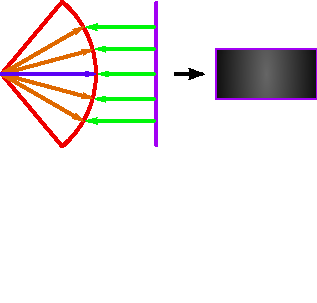
\includegraphics[width=0.5\textwidth]{additional/fisheye1.pdf}
		\caption{Демонстрация эффекта}
	\end{figure}

	Такой эффект носит название эффекта <<рыбьего глаза>>. Для исправления такого эффекта необходимо, чтобы длина проекции на направляющий вектор каждого отклоненного вектора c некоторым коэффициентом масштабирования \( \tilde{v}_{ij} = k v_{ij} \) совпадала с длиной самого направляющего вектора:
	\[ \abs{\Pr\pares{\tilde{v}_{ij}, v}} \equiv \abs{v}. \]
	Таким образом необходимо найти такое значение $k$, при котором это условие выполняется.

	Положим, что угол между векторами $v$ и \( v_{ij} \) в пространстве равен \( \gamma \). Тогда:
	\[ \abs{\Pr\pares{v_{ij}, v}} = \abs{v} \cos{\gamma}, \]
	при этом
	\( \abs{\tilde{v}_{ij}} = \abs{k} \cdot \abs{v_{ij}} \), и по свойству оператора проецирования \( \abs{\Pr\pares{\tilde{v}_{ij}, v}} = \abs{\Pr\pares{k \cdot v_{ij}, v}} = \abs{k} \cdot \abs{\Pr\pares{v_{ij}, v}} \). Разделяя на \( \cos{\gamma} \), получим коэффициент масштабирования:
	\[ k = \sec{\gamma} \implies \tilde{v}_{ij} = v_{ij} \cdot \sec{\gamma}. \]
	Угол между двумя векторами можно получить из формулы скалярного произведения двух векторов:
	\[ \pares{v, v_{ij}} = \abs{v} \cdot \abs{v_{ij}} \cdot \cos{\gamma} \implies \sec{\gamma} = \frac{\abs{v} \cdot \abs{v_{ij}}}{\pares{v, v_{ij}}} = \frac{\abs{v}^2}{\pares{v, v_{ij}}}. \]

	Таким образом,
	\[ \tilde{v}_{ij} = v_{ij} \sec{\gamma} = \frac{\abs{v}^2}{\pares{v, v_{ij}}} \cdot v_{ij}. \]

	Полученный результат можно проиллюстрировать на следующем изображении:
	\begin{figure}[H]
		\centering
		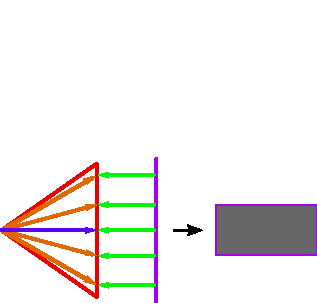
\includegraphics[width=0.5\textwidth]{additional/fisheye2.pdf}
		\caption{Метод исправления полученного эффекта}
	\end{figure}

	Здесь может возникнуть ситуация, когда \( \pares{v, v_{ij}} = 0 \). Она может возникнуть в том случае, если вектора ортогональны друг другу, что может возникнуть при условии, что углы обзора содержат в себе значения, не меньшие $\pi$. Соответственно, такой угол не является допустимым в рамках данной реализации. 


\subsection{Класс Ray}
	\noindent Реализуемые методы:
	\begin{enumerate}
		\item \inlinecode{normalize()} -- метод, выполняющий нормировку направляющего вектора в луче.
	\end{enumerate}


\subsection{Класс Game.Object}
	\noindent Реализуемые методы:
	\begin{enumerate}
		\item \inlinecode{intersection_distance(ray: Ray) -> float} -- метод поиска расстояния от начала луча до точки пересечения луча с объектом. В глобальном классе считается пустым методом, возвращающим по умолчанию \inlinecode{0}. Для каждого объекта задается индивидуально.
	\end{enumerate}


\subsection{Класс Game.Camera[\textit{Game.Object}]}
	Для камеры необходимо прописать метод рассчета лучей, полученных путем алгоритма, описанного выше:

	\noindent Реализуемые методы:
	\begin{enumerate}
		\item \inlinecode{get_rays_matrix(n, m: int) -> Matrix\{n, m\}[[Ray]]} -- метод, с помощью которого получаются все возможные лучи.
	\end{enumerate}

	Данный метод может работать корректно только в случае, когда камера является камерой с направляющим обзор вектором (\inlinecode{direction}). В случае, если камера задается точкой обзора (\inlinecode{look_at}), необходимо обработать такой случай отдельно, и вычислить нормированный направляющий вектор по двум точкам -- позиция камеры и точка обзора.


\subsection{Класс Game.HyperPlane[\textit{Game.Object}]}
	Здесь необходимо перейти к модулю, описывающему уже конкретную игру, и создать в нем объект плоскости.

	\noindent Инициализация:
	\begin{enumerate}
		\item \inlinecode{Game.HyperPlane(position: Point, normal: Vector)} -- класс гиперплоскости, заданной в некотором положении в заданной системе координат с вектором нормали к гиперплоскости. При инициализации вызывается метод \inlinecode{set_property} для заданных аргументов. Вектор направления необходимо нормировать в заданном векторном пространстве.
	\end{enumerate}

	\noindent Перегружаемые методы:
	\begin{enumerate}
		\item \inlinecode{planar_rotate(inds: (int, int), angle: float) -> None} -- повернуть нормаль гиперплоскости в пространстве.
		\item \inlinecode{rotate_3d(angles: (float, float, float)) -> None} -- повернуть трехмерную плоскость на заданные углы;
		\item \inlinecode{intersection_distance(ray: Ray) -> float} -- метод нахождения расстояния от начала луча до точки пересечения плоскости и луча.
	\end{enumerate}


\subsection{Класс Game.HyperEllipsoid[\textit{Game.Object}]}

	\noindent Инициализация:
	\begin{enumerate}
		\item \inlinecode{Game.HyperEllipsoid(position: Point, direction: Vector, semiaxes: list[float])} -- класс гиперэллипса, заданного в некотором положении в заданной системе координат, повернутый по заданному вектору направления, с соответствующими $n$-полуосями.
	\end{enumerate}

	\noindent Перегружаемые методы:
	\begin{enumerate}
		\item \inlinecode{planar_rotate(inds: (int, int), angle: float) -> None} -- повернуть гиперэллипс в пространстве.
		\item \inlinecode{rotate_3d(angles: (float, float, float)) -> None} -- повернуть трехмерный эллипсоид на заданные углы;
		\item \inlinecode{intersection_distance(ray: Ray) -> float} -- метод нахождения расстояния от начала луча до точки пересечения гиперэллипса и луча.
	\end{enumerate}


\subsection{Класс Game.Canvas}

	Данный класс описывает базовый <<холст>> для отрисовки. Уже содержит в себе всю информацию об игре (список сущностей, систему координат).

	\noindent Инициализация:
	\begin{enumerate}
		\item \inlinecode{Game.Canvas(n, m: int)} -- размер экрана.
	\end{enumerate}

	\noindent Реализуемые поля:
	\begin{enumerate}
		\item \inlinecode{n(int), m(int)} -- размерность экрана;
		\item \inlinecode{distances(Matrix\{n, m\}[[float]])} -- матрица расстояний. Необходима для отрисовки.
	\end{enumerate}

	\noindent Реализуемые методы:
	\begin{enumerate}
		\item \inlinecode{draw() -> None} -- метод, производящий отрисовку в классе \inlinecode{Game} известной матрицы \inlinecode{distances};
		\item \inlinecode{update(camera: Game.Camera) -> None} -- метод, обновляющий матрицу \inlinecode{distances} согласно виду из камеры. Производит полный пробег по всем сущностям \inlinecode{EntityList}, на основе которых с помощью метода \inlinecode{intersection_distance} строит новую матрицу \inlinecode{distances}.
	\end{enumerate}


\subsection{Этапы реализации}

	Зафиксируем представленные классы в поэтапной реализации движка:
	\begin{enumerate}
		\item Сформируем логическую структуру файлов в проекте;
		\item Реализуем рассчет и отправку лучей из камеры с учетом разрешения эффекта <<рыбьего глаза>>;
		\item Введем несколько дополнительных методов для класса луча и игрового объекта;
		\item Внутри игры создадим два наследуемых игровых объекта -- гиперплоскость и гиперэллипс, для которых пропишем методы пересечения с лучем;
		\item Создадим класс полотна, которое в дальнейшем будем использовать для отрисовки объектов.
	\end{enumerate}



	\pagebreak
	\section{Лабораторная работа №5: Обработка событий и отрисовка}
	В пятой лабораторной работе мы займемся отрисовкой графики в консоли, реализацией системы событий, и системой настроек.

\subsection{Система событий}
	
	Рассматривать будем примитивную систему событий, в которой будет только вызов и обработка событий в некотором пространстве событий. Сама система событий представляет собой систему обмена информацией между независимыми объектами, и задается в каждом объекте класса \inlinecode{Game} индивидуально. События можно вызывать с некоторыми параметрами, которые отлавливаются самой системой, и обрабатываются.

	Работа производится по следующему принципу:
	\begin{enumerate}
		\item Произвольная сущность вызывает событие с некоторыми аргументами;
		\item Обработчик событий вызывает функции, отвечающие за данное событие с предоставленными ему аргументами.
	\end{enumerate}
	% Для конкретных событий существует массив функций, которые вызываются последовательно внутри игры с аргументами, переданными обработчику. 
	В данном варианте системы событий, обращение к обработчику производится по имени события.

	Рассмотрим следующий пример. Положим, что существует объект \inlinecode{sphere}, который при перемещении камеры игрока \inlinecode{player} двигается вместе с ним. Для камеры существует обработчик нажатия на клавиши перемещения. Введем новое событие (\inlinecode{Game.Event.add}) в систему под названием \inlinecode{\"OnMainCameraMove\"}. Для данного события добавим функцию-обработчик (\inlinecode{Game.Event.handle}), которая принимает на себя в качестве аргументов сущность игрока, и меняет положение сферы. Затем вызовем событие (\inlinecode{Game.Event.trigger}) в методе перемещения камеры, где в качестве аргумента передадим саму камеру. Будем подразумевать, что при вызове события, вызовется его обработчик с аргументом, переданным в функции вызова:

	\begin{figure}[H]
\begin{lstlisting}[caption=Пример кода реализации описанного алгоритма событий]
in Game.init:
	sphere = Game.HyperSphere(Point(0, 0, 0), Vector(1, 0, 0))

	def handler(camera: Game.Entity):
		sphere.set_position(camera.get_position())

	Game.Event.add("OnMainCameraMove")
	Game.Event.handle("OnMainCameraMove", handler)

in Game.camera.movement:
	Game.Event.trigger("OnMainCameraMove", camera)
\end{lstlisting}
	\end{figure}


\subsection{Игровые параметры}
	
	Рассмотрим концепцию параметров игры. Введем в игру конфигурационный файл, содержащий в себе базовую информацию для настроек игры. К настройкам игры можно отнести управление, дальность прорисовки, размеры экрана, и другие значения. 

	Конфигурационный файл можно хранить в любом удобном формате. Все константные значения можно на данном этапе перенести в этот файл, поместив его в папку \inlinecoden{config/}, с названием, к примеру, \inlinecode{default.*} или \inlinecode{autoexec.*} (файл с расширением <<удобного>> формата).

	В концепцию параметров игры включим возможность подключать несколько конфигурационных файлов, которые будут вызываться последовательно. Для них разрешается перезаписывать данные, которые уже были записаны в других файлах.
	

\subsection{Класс EventSystem}
	
	\noindent Класс, отвечающий за реализацию и обработку события. Является независимым классом.

	\noindent Инициализация:
	\begin{enumerate}
		\item \inlinecode{EventSystem()} -- класс системы событий. Содержит в себе информацию о существующих событиях в игре.
	\end{enumerate}

	\noindent Реализуемые поля:
	\begin{enumerate}
		\item \inlinecode{events(dict[str: list[Callable]])} -- таблица информации о событиях. Ключем является имя события, значением -- массив вызываемых функций, каждая из которых принимает одно и то же число аргументов;
	\end{enumerate}

	\noindent Реализуемые методы:
	\begin{enumerate}
		\item \inlinecode{add(name: str)} -- метод, добавляющий в систему событий новое имя для события;
		\item \inlinecode{remove(name: str)} -- метод, удаляющий из системы событий заданное имя;
		\item \inlinecode{handle(name: str, function: Callable)} -- метод, добавляющий функцию-обработчик в массив функций для заданного имени события;
		\item \inlinecode{remove_handled(name: str, function: Callable)} -- метод, удаляющий функцию-обработчик из массива функций для заданного имени события;
		\item \inlinecode{trigger(name: str, *args)} -- метод, вызывающий в пространстве событий все функции-обработчики для заданного имени события с переданными аргументами;
		\item \inlinecode{get_handled(name: str)} -- метод, возвращающий все функции-обработчики для заданного события.
	\end{enumerate}

	\noindent Перегружаемые операторы:
	\begin{enumerate}
		\item \inlinecode{EventSystem[name: str]} (операция, возвращающая все функции-обработчики для заданного события, не имеет возможности установки значений).
	\end{enumerate}


\subsection{Класс Game.Configuration}

	Класс, содержащий информацию о значениях параметров, подключенных из отдельного файла. Параметры можно редактировать и подключать во время исполнения.

	\noindent Инициализация:
	\begin{enumerate}
		\item \inlinecode{Game.Configuration()} -- общий класс конфигурации игры;
		\item \inlinecode{Game.Configuration(filepath: str)} -- класс конфигурации игры, содержащий в себе информацию о константах или переменных из файла.
	\end{enumerate}

	\noindent Реализуемые поля:
	\begin{enumerate}
		\item \inlinecode{filepath(str)} -- строка пути к конфигурационному файлу. Может быть пустой строкой;
		\item \inlinecode{configuration(dict[str: any])} -- таблица подгруженных значений переменных из конфигурационного файла. В случае отсутствия файла, подгружает значение по умолчанию.
	\end{enumerate}

	\noindent Реализуемые методы:
	\begin{enumerate}
		\item \inlinecode{set_variable(var: str, value: any | None) -> None} -- метод, устанавливающий (или удаляющий) значение переменной в текущей конфигурации;
		\item \inlinecode{get_variable(var: str) -> any} -- метод, возвращающий значение переменной в текущей конфигурации;
		\item \inlinecode{execute_file(filepath: str)} -- метод, обновляющий значения переменных, подгруженных из файла;
		\item \inlinecode{save(filepath: str)} -- метод, сохраняющий конфигурацию в файл. В случае, если файл не указан, сохраняет в файл с именем файла из поля \inlinecode{filepath} текущей конфигурации. В случае, если файлы не указаны как в аргументе, так и в поле, вызывать ошибку невозможности сохранения файла.
	\end{enumerate}

	\noindent Перегружаемые операторы:
	\begin{enumerate}
		\item \inlinecode{Game.Configuration[var: str]} (оператор обращения (и присваивания) параметру значений).
	\end{enumerate}


\subsection{Класс Game}
	Для класса \inlinecode{Game} необходимо добавить в инициализацию систему событий, которая в дальнейшем будет использоваться для взаимодействия между сущностями.

	\noindent Инициализация:
	\begin{enumerate}
		\item \inlinecode{Game(cs: CoordinateSystem, es: EventSystem, entities: EntitiesList)} -- класс игры, содержащий в себе базовую информацию в виде системы координат, подключенной системы событий и списка сущностей.
	\end{enumerate}

	\noindent Реализуемые поля:
	\begin{enumerate}
		\item \inlinecode{es(EventSystem)} -- реализуемая система событий в данном экземпляре игры;
	\end{enumerate}

	\noindent Реализуемые методы:
	\begin{enumerate}
		\item \inlinecode{get_event_system() -> EventSystem} -- метод, возвращающий объект класса системы событий для данного экзмепляра игры;
		\item \inlinecode{apply_configuration(configuration: Game.Configuration)} -- метод, применяющий параметры конфигурационного файла в игре (изменяет переменные).
	\end{enumerate}


\subsection{Класс Game.Console[\textit{Game.Canvas}]}
	
	Введем класс для отрисовки изображения в консоли. Реализацию можно проводить на любом доступном движке консольной отрисовке, например, на движке \inlinecode{ncurses}.

	\noindent Реализуемые поля:
	\begin{enumerate}
		\item \inlinecode{Game.Console.charmap(list[str]))} -- список символов, расположенных в порядке увеличения/уменьшения заполняемого символом объема.
		Классический пример:
\begin{lstlisting}
charmap = ".:;><+r*zsvfwqkP694VOGbUAKXH8RD#$B0MNWQ%&@"
\end{lstlisting}
		Также, эти символы можно перенести в конфигурационный файл, опционально.
	\end{enumerate}

	\noindent Реализуемые методы:
	\begin{enumerate}
		\item \inlinecode{draw() -> None} -- метод, производящий отрисовку в классе \inlinecode{Game} известной матрицы \inlinecode{distances} в консоль с использованием библиотеки отрисовки и символов, заданных в данном классе.
	\end{enumerate}


\subsection{Дополнительно}

	В данной работе требуется реализовать также управление камерой в пространстве. Рассматривать будем трехмерное пространство, движение возможно по шести направлениям -- вперед, назад, влево, вправо (без вращения камеры), вверх и вниз (клавишами \inlinecoden{space}, \inlinecoden{ctrl}). Поворот камеры осуществляется в двумерном пространстве -- вращение в горизонтальной плоскости \( XY \), и вертикальной, пересекающей камеру по центру (в плоскости направляющего вектора и вектора, отвечающего за ось $z$). Для поворота можно обозначить клавиши <<стрелочки>> -- повороты влево, вправо, вверх и вниз.


\subsection{Этапы реализации}

	Зафиксируем представленные классы в поэтапной реализации движка:
	\begin{enumerate}
		\item Реализуем класс системы событий, способный обрабатывать события для игры, и пропишем его при инициализации игры;
		\item Добавим в игру понятие параметров, в которые запишем все возможные константы или переменные (параметры) игры;
		\item Добавим класс отрисовки в консоль на основе класса <<полотна>> игры;
		\item Добавим возможность управления камерой с помощью клавиатуры. Движения должны обрабатываться системой событий, когда игра отлавливает нажатия на клавиши, передает событие перемещения, а камера обрабатывает событие, совершая действия.
	\end{enumerate}

\end{document}